\chapter{Návrh architektury} \label{chap:architektura}

Tato kapitola se zabývá návrhem architektury systému aplikace pro sběr dat o IEQ. Návrh vychází z identifikovaných požadavků a případů užití vymezených v předchozích kapitolách.  

Na obrázku č. \ref{fig:archimate-model} lze vidět celkový pohled na model. Model je však rozsáhlý a pro nejlepší zážitek z prohlížení byla vytvořena webová stránka \href{archimate.ambiquality.org}{archimate.ambiqulity.org}, kde lze model podrobně prohlížet. Stránka byla vygenerována pomocí funkce \textit{Report -> HTML} v aplikaci \textit{Archi}, která byla pro modelování použita.

\begin{figure}[hbtp!]
  \centering
  \caption{Celkový model architektury}
  \label{fig:archimate-model}
  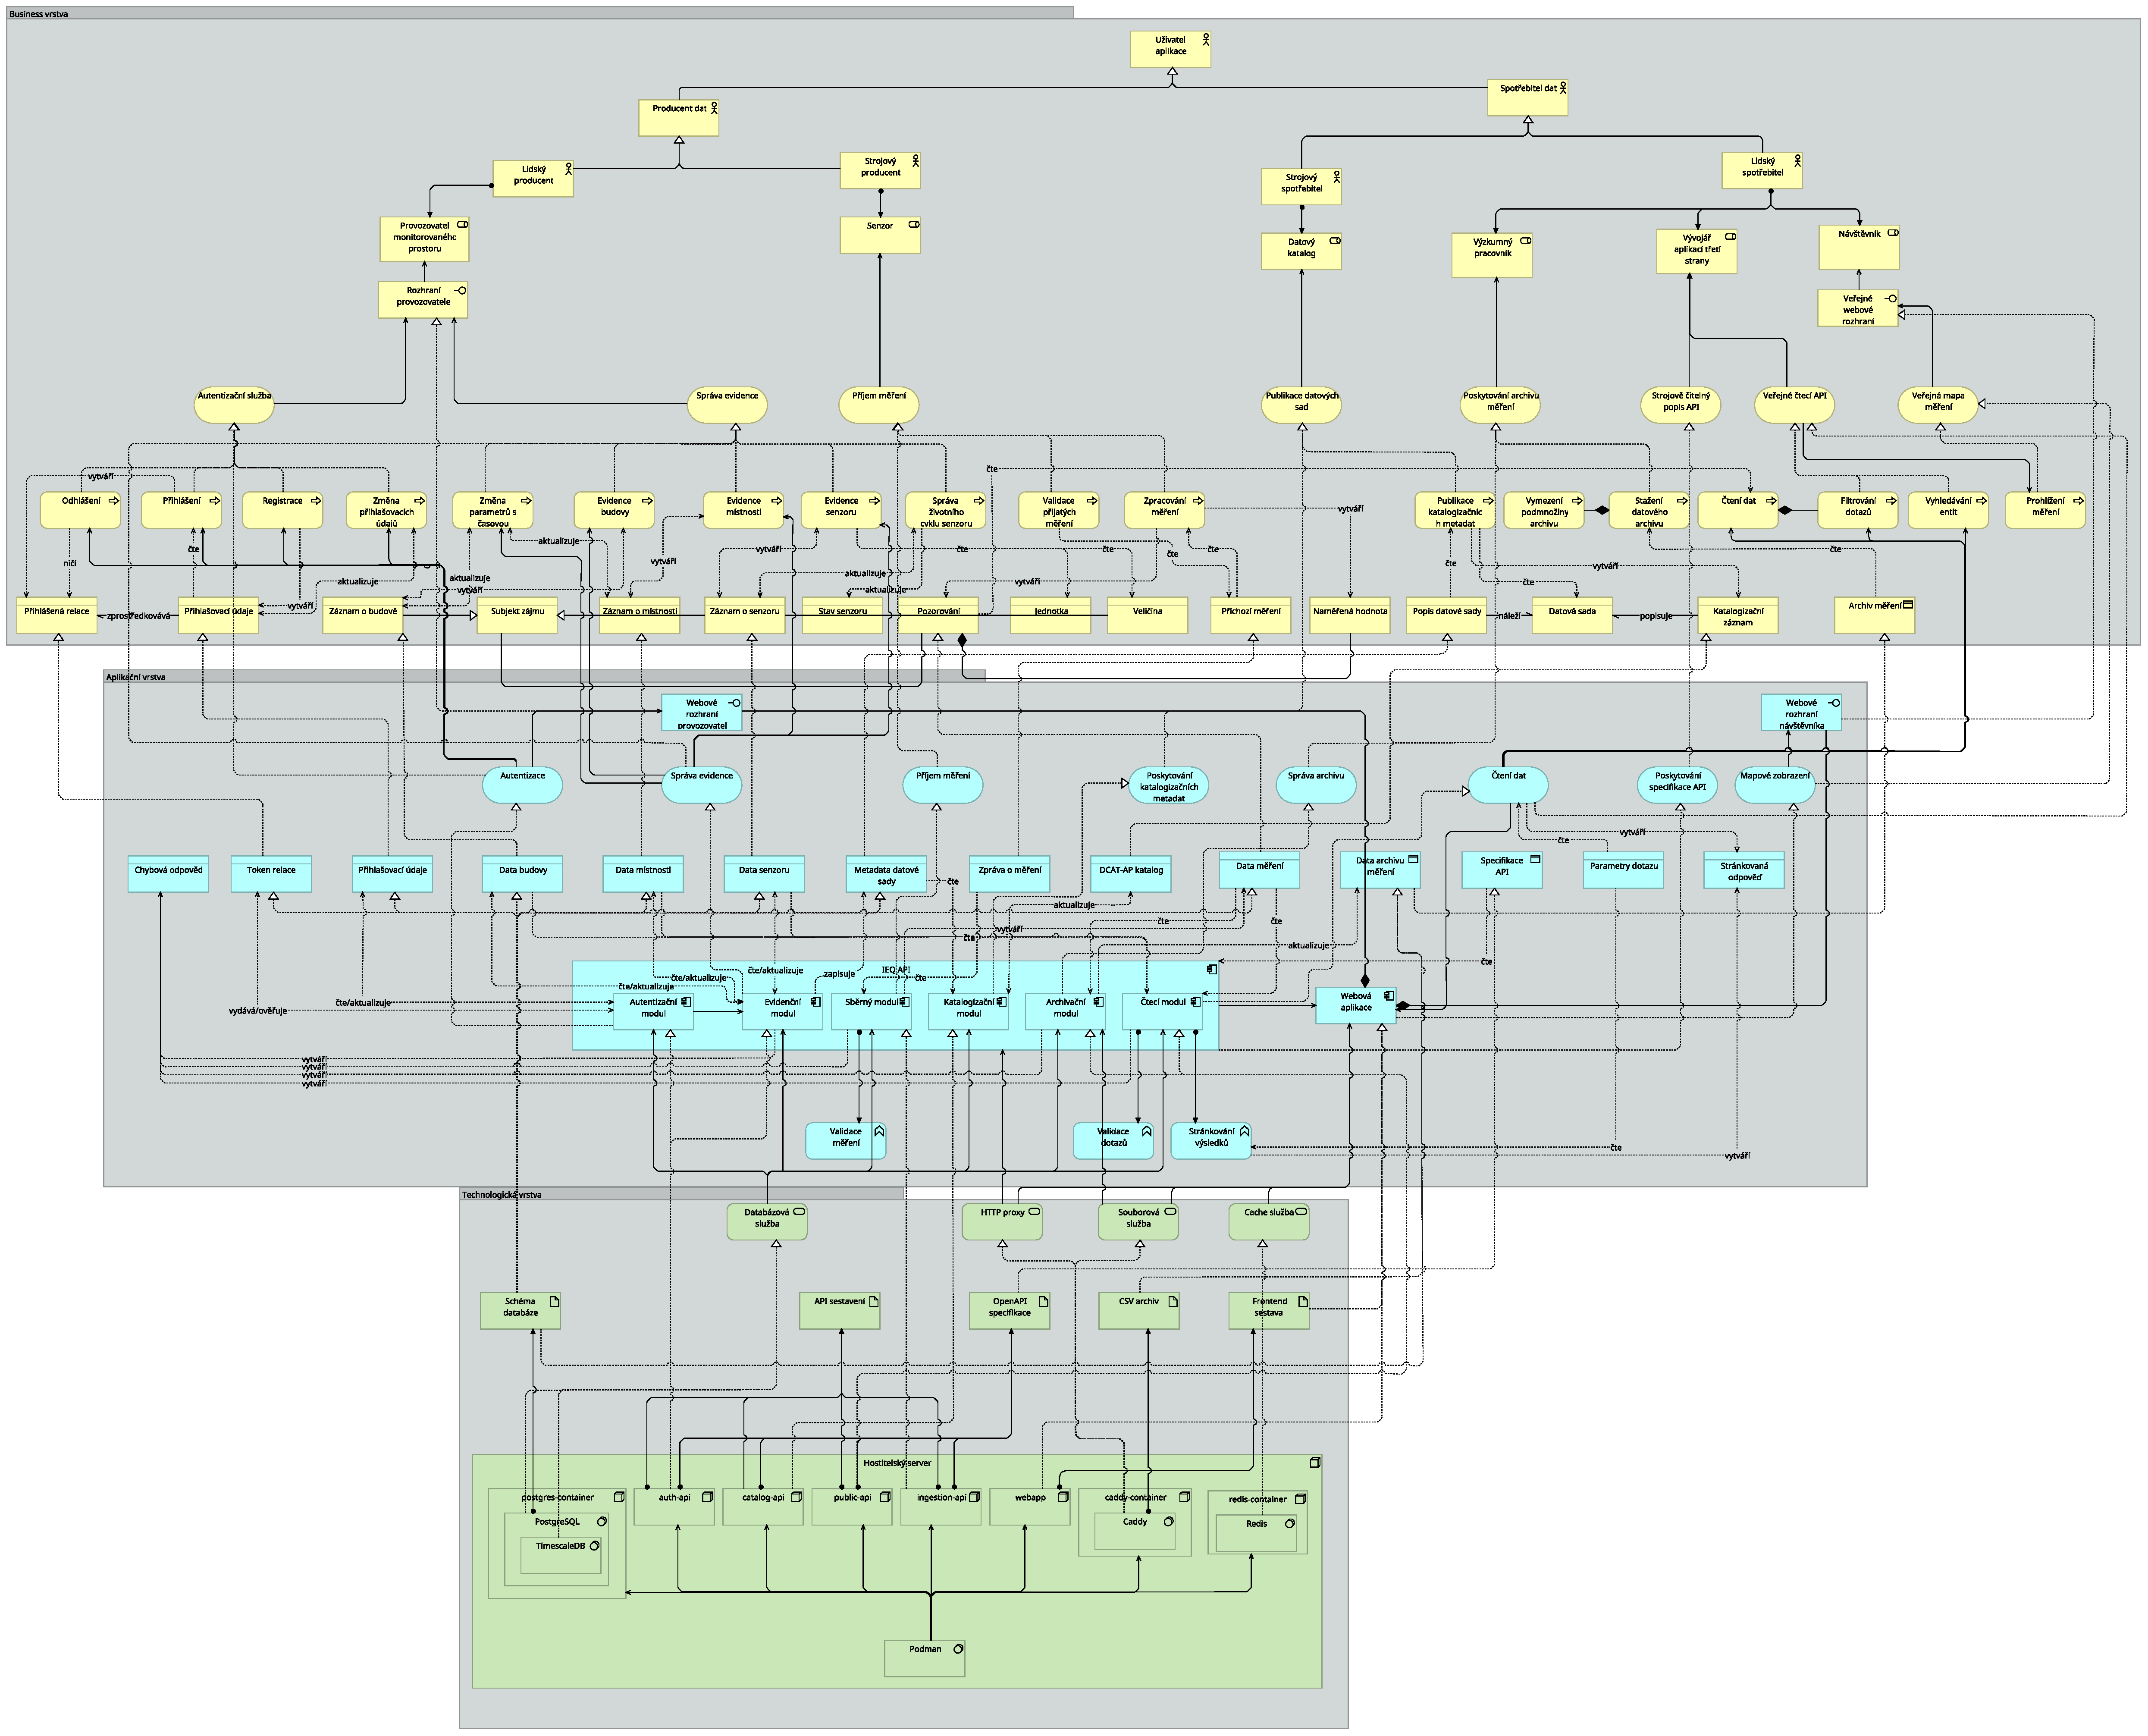
\includegraphics[width=0.9\textwidth]{img/model}

  \scriptsize \textit{Zdroj:} Vlastní zpracování
\end{figure}

\section{Business vrstva}

Business vrstva, zachycená na obrázku č.~\ref{fig:archimate-business-layer}, popisuje organizační kontext systému prostřednictvím aktérů, rolí, služeb a procesů. Aktéři jsou hierarchicky uspořádáni: kořenový aktér \textit{Uživatel aplikace} se větví na \textit{Producenta dat} a \textit{Spotřebitele dat}, přičemž každý z nich má lidskou a strojovou variantu (tzn. senzor jako strojový producent). Listoví aktéři jsou přiřazeni k odpovídajícím rolím – \textit{Provozovatel monitorovaného prostoru}, \textit{Návštěvník}, \textit{Výzkumný pracovník} a \textit{Vývojář aplikací třetí strany} – které nesou odpovědnosti za konkrétní chování v systému.

Klíčové byznys služby zahrnují správu evidence prostoru a senzorů, příjem měření, veřejnou mapu měření, veřejné čtecí API a poskytování datového archivu. Tyto služby jsou realizovány byznys procesy jako \textit{Přihlášení}, \textit{Registrace}, \textit{Příjem měření} nebo \textit{Prohlížení měření}. Jako sdílené byznys objekty vystupují zejména \textit{Měření}, \textit{Data budovy}, \textit{Data místnosti} a \textit{Data senzoru}.

\begin{figure}[hbtp!]
  \centering
  \caption{Model obchodní vrstvy}
  \label{fig:archimate-business-layer}
  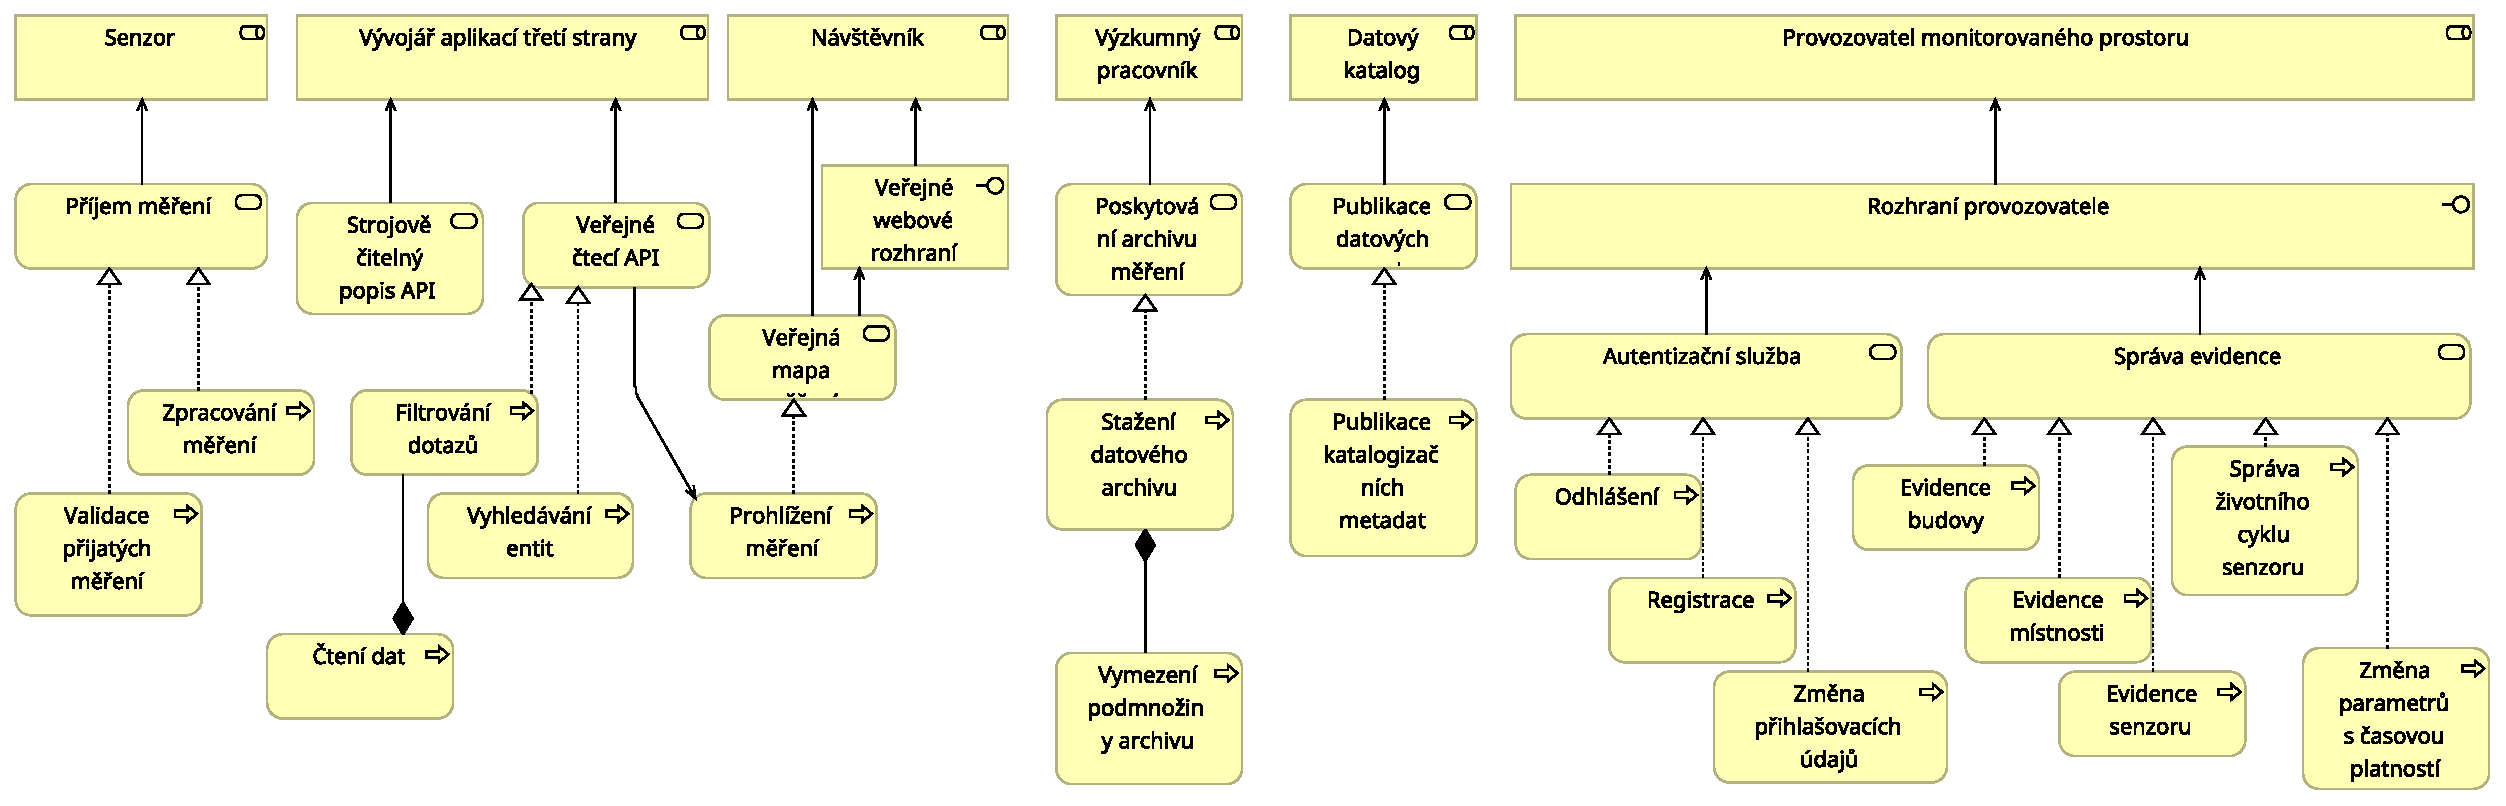
\includegraphics[width=0.9\textwidth]{img/business-layer}

  \scriptsize \textit{Zdroj:} Vlastní zpracování
\end{figure}

\section{Aplikační vrstva}

Aplikační vrstva, zobrazená na obrázku č.~\ref{fig:archimate-app-layer}, modeluje softwarové komponenty a jejich vzájemné vztahy. Centrálním prvkem je komponenta \textit{IEQ API}, která zastřešuje šest specializovaných modulů: \textit{Autentizační}, \textit{Evidenční}, \textit{Sběrný}, \textit{Čtecí}, \textit{Katalogizační} a \textit{Archivační}. Každý modul realizuje skupinu aplikačních služeb odpovídající příslušným funkčním požadavkům – například Sběrný modul poskytuje služby příjmu a validace příchozích měření, Čtecí modul zajišťuje stránkování a filtrování dotazů.

Druhou hlavní komponentou je \textit{Webová aplikace}, která agreguje dvě aplikační rozhraní: \textit{We-bo-vé rozhraní provozovatele} a \textit{Webové rozhraní návštěvníka}. Obě rozhraní jsou vystavena jedinou single-page aplikací a realizují odpovídající byznys rozhraní z vrstvy níže. Datové objekty (např. \textit{Specifikace API}, \textit{Token relace} nebo \textit{Parametry dotazu}) dokumentují klíčové informační artefakty procházející vrstvou.

\begin{figure}[hbtp!]
  \centering
  \caption{Model aplikační vrstvy}
  \label{fig:archimate-app-layer}
  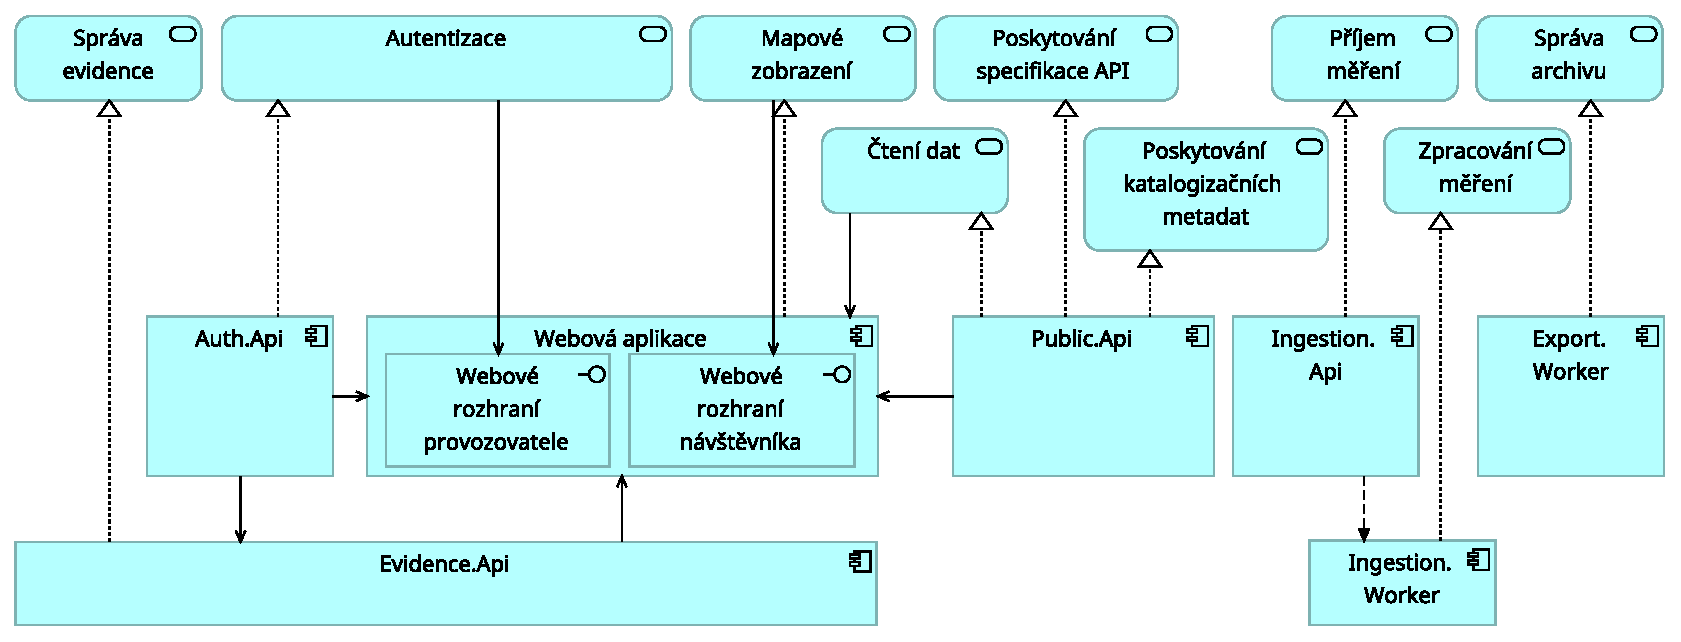
\includegraphics[width=0.9\textwidth]{img/app-layer}

  \scriptsize \textit{Zdroj:} Vlastní zpracování
\end{figure}

\section{Technologická vrstva}

Technologická vrstva, zachycená na obrázku č.~\ref{fig:archimate-tech-layer}, popisuje nasazení systému na infrastrukturní úrovni. Veškeré komponenty jsou provozovány na jediném \textit{Hostitelském serveru}, který obsahuje kontejnerový engine \textit{Podman}. Pod ním jsou kompozičně zanořeny kontejnerové uzly odpovídající jednotlivým službám: \textit{auth-api}, \textit{ingestion-api}, \textit{public-api}, \textit{catalog-api} a \textit{webapp} pro aplikační složky, dále \textit{postgres-container}, \textit{redis-container} a \textit{caddy-container} pro podpůrnou infrastrukturu.

Systémový software zahrnuje \textit{PostgreSQL} s rozšířením \textit{TimescaleDB} pro časové řady měření, \textit{Redis} jako cache vrstvu a \textit{Caddy} jako HTTP proxy zajišťující ingress. Technologické služby (\textit{Databázová služba}, \textit{Cache služba}, \textit{Souborová služba}) abstrahují přístup k persistentním uložištím. Artefakty jako \textit{Frontend sestava} nebo \textit{CSV archiv} reprezentují nasaditelné výstupy sestavení.

\begin{figure}[hbtp!]
  \centering
  \caption{Model technologické vrstvy}
  \label{fig:archimate-tech-layer}
  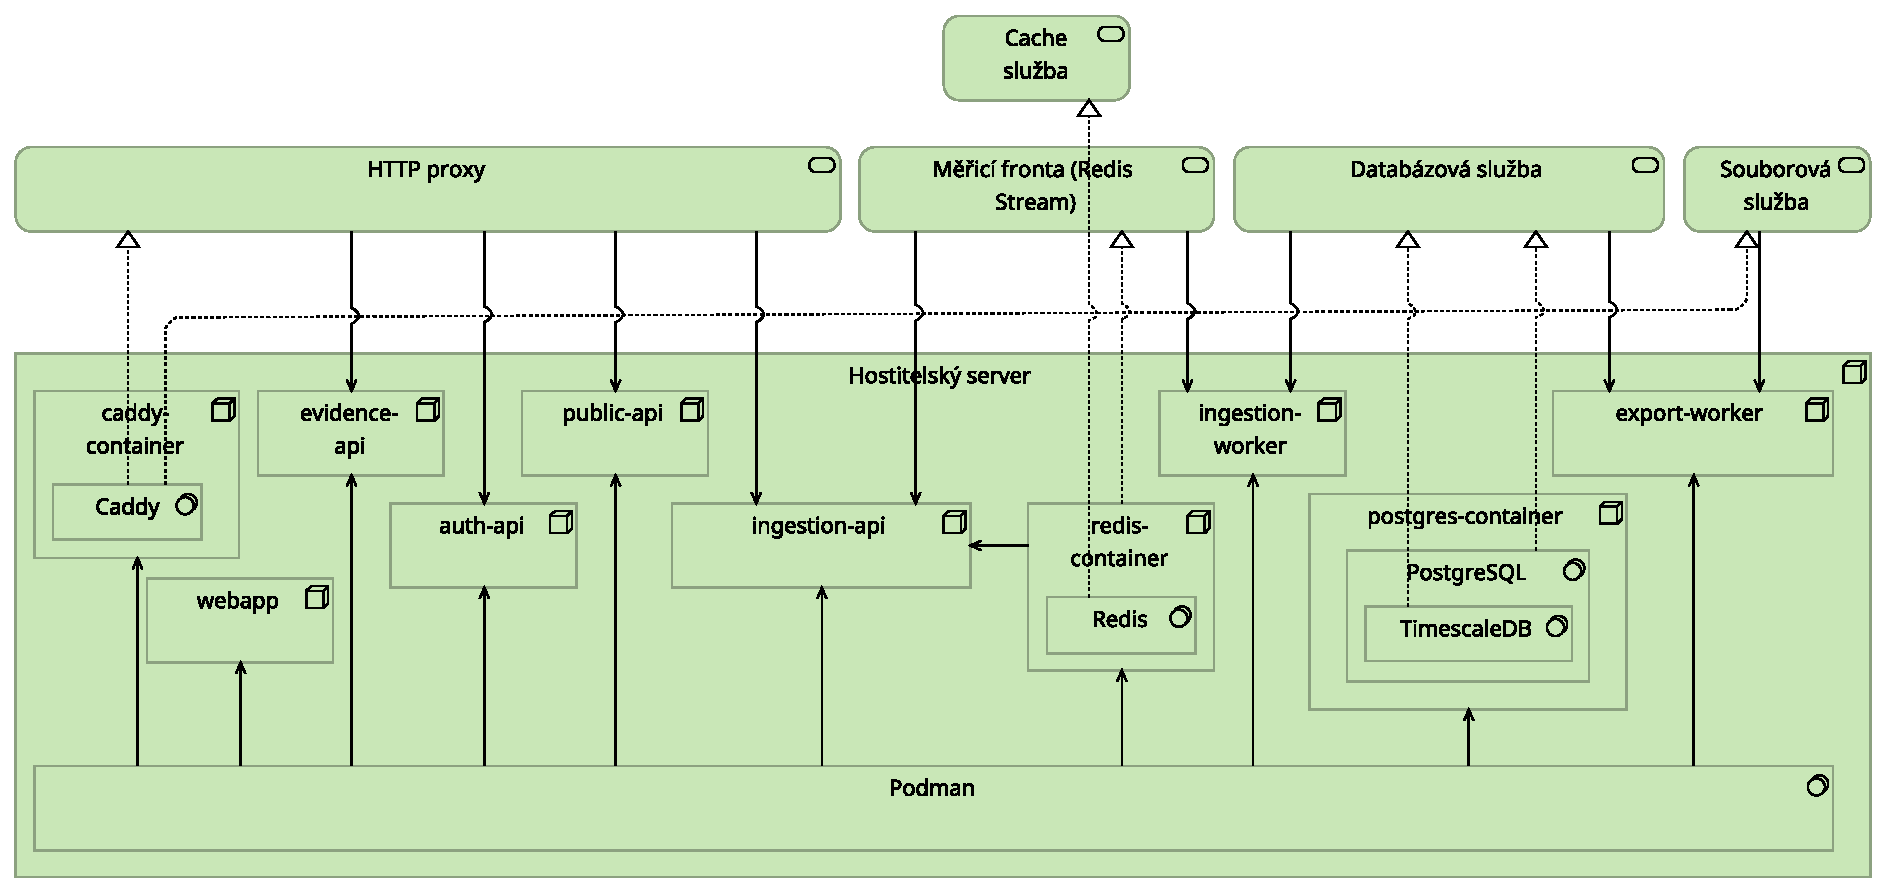
\includegraphics[width=0.9\textwidth]{img/tech-layer}

  \scriptsize \textit{Zdroj:} Vlastní zpracování
\end{figure}
